\documentclass[tikz]{standalone}
\usepackage{tikz}
\usetikzlibrary{positioning, graphs}
\usetikzlibrary{graphs.standard}
\begin{document}
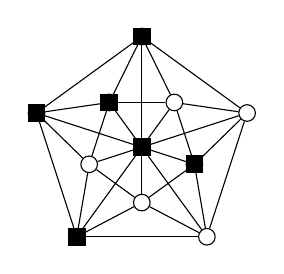
\begin{tikzpicture}
    [circle_node/.style={circle, draw, inner sep = 0, minimum size = 0.6em},
     rectangle_node/.style={rectangle, draw, inner sep = 0, minimum size = 0.6em, fill=black}]

    \graph[clockwise, radius=4em, phase=18, empty nodes, nodes=circle_node]{subgraph C_n[n = 5, name = A]};
    \graph[clockwise, radius=2em, phase=-18, empty nodes, nodes=circle_node]{subgraph C_n[n = 5, name = B]};
    \node[rectangle_node] (center) at (0, 0) {};

    \foreach \i [evaluate={\j=int(mod(\i,5)+1)}] in {1,...,5}{
		\draw (A \i) -- (B \i);
        \draw (A \j) -- (B \i);
        \draw (A \i) -- (center);
        \draw (B \i) -- (center);
    }

    \node[rectangle_node] (a) at (A 3) {};
    \node[rectangle_node] (b) at (A 4) {};
    \node[rectangle_node] (c) at (A 5) {};
    \node[rectangle_node] (d) at (B 4) {};
    \node[rectangle_node] (e) at (B 1) {};
\end{tikzpicture}
\end{document}